\documentclass[conference]{IEEEtran}
% High-Swing Cascode Current Mirror -- gpdk090. Figures in this directory:
% fig_sch.png fig_cmp.png fig_vout.png fig_rout.png fig_tran.png fig_vdd.png
% fig_layf.png fig_laym.png
\usepackage{graphicx}
\usepackage{booktabs}
\usepackage{siunitx}
\usepackage[hidelinks]{hyperref}
\sisetup{detect-all}

\begin{document}

\title{Design, Simulation and Physical Verification of a\\ High-Swing Cascode Current Mirror}

\author{\IEEEauthorblockN{Somya Bhura (23BEC187)}
\IEEEauthorblockA{Department of Electronics and Communication Engineering\\
Institute of Technology\\
Academic Year 2026--2027, Semester VII}}

\maketitle

\begin{abstract}
This paper presents the design and simulation of a high-swing (wide-swing)
cascode current mirror that overcomes the low output resistance of a simple
current mirror and the high voltage-headroom requirement of a conventional
cascode mirror, while maintaining stable \SI{100}{\micro\ampere} operation at
a \SI{1.8}{\volt} supply. The circuit is implemented in Cadence Virtuoso with
the GPDK090 library using five NMOS transistors (mirror devices
$W=\SI{12}{\micro\metre}$, $L=\SI{1}{\micro\metre}$; bias device
$W=\SI{3}{\micro\metre}=W/4$), with the cascode gates biased at
$V_{TH}+2V_{ov}$ by the quarter-width diode device. Simulation shows an
output current of \SI{100.06}{\micro\ampere}, an output resistance of
\SI{1.57}{\mega\ohm} ($13\times$ the simple mirror's \SI{0.12}{\mega\ohm}),
and 99\% current compliance at only \SI{0.44}{\volt} of output voltage ---
\SI{0.35}{\volt} less headroom than the conventional cascode's
\SI{0.79}{\volt}. A full custom layout was drawn and verified: Diva DRC
reports zero errors and LVS matches the schematic exactly. A side-by-side
sweep of all three mirror topologies quantifies the trade-offs.
\end{abstract}

\begin{IEEEkeywords}
Cascode current mirror, wide-swing, high-swing, output resistance, voltage
headroom, Cadence Virtuoso, GPDK090, DRC, LVS.
\end{IEEEkeywords}

\section{Introduction}
A simple two-transistor current mirror has an output resistance of only
$r_o = 1/\lambda I_D$, so its output current varies appreciably with output
voltage --- a serious limitation when the mirror biases high-gain stages
\cite{gray,razavi}. Cascoding multiplies the output resistance by
$g_m r_o$, but the conventional cascode connection, which biases the cascode
gate from a stacked diode pair, wastes headroom: its minimum output voltage
is $V_{TH}+2V_{ov}$, a full threshold voltage more than the physical limit of
two saturation voltages.

The high-swing (wide-swing) cascode mirror, attributed to Sooch \cite{sooch},
removes this waste. A separate bias device of width $W/4$ --- carrying the
same reference current at twice the overdrive --- generates
$V_B \approx V_{TH}+2V_{ov}$ for the cascode gates, while the mirror gates
are driven from the input node. The bottom devices then sit at
$V_{DS}\approx V_{ov}$, the edge of saturation, and the output complies down
to about $2V_{ov}$. This work designs the circuit at \SI{100}{\micro\ampere}
and \SI{1.8}{\volt} in GPDK090, verifies it against the BSIM3v3 models,
compares all three topologies in one simulation, and carries the design
through layout, DRC and LVS.

\section{Circuit Configuration and Design}

\subsection{Topology}
The circuit (Fig.~\ref{fig:sch}) contains five NMOS devices. M0
($W=\SI{3}{\micro\metre}$) is diode-connected and fed by
$I_0=\SI{100}{\micro\ampere}$; its gate voltage $V_B$ drives the gates of the
cascode devices M3 and M4. The input branch stacks cascode M3 on mirror
device M1; the gates of M1 and M2 are tied to the input node (the wide-swing
connection), not to M1's drain. The output branch stacks M4 on M2. All mirror
and cascode devices use $W=\SI{12}{\micro\metre}$, $L=\SI{1}{\micro\metre}$.
The output is exercised by a swept/AC source V2. The design values are
summarized in Table~\ref{tab:spec}.

\begin{table}[!t]
\caption{Design Specifications}
\label{tab:spec}
\centering
\begin{tabular}{ll}
\toprule
Parameter & Value \\
\midrule
Supply voltage, $V_{DD}$ & \SI{1.8}{\volt} \\
Reference currents $I_0$, $I_1$ & \SI{100}{\micro\ampere} each \\
Mirror/cascode devices M1--M4 & $W=\SI{12}{\micro\metre}$, $L=\SI{1}{\micro\metre}$ \\
Bias device M0 & $W=\SI{3}{\micro\metre}=W/4$, $L=\SI{1}{\micro\metre}$ \\
Technology & GPDK090, nmos2v, BSIM3v3 \\
Output test source & DC sweep + \SI{100}{\milli\volt}, \SI{1}{\kilo\hertz} sine \\
\bottomrule
\end{tabular}
\end{table}

\subsection{Bias design}
With $I_D = \tfrac12 \mu_n C_{ox}(W/L)V_{ov}^2$, quartering $W$ at constant
current doubles the overdrive. M0 therefore develops
$V_{GS0}=V_{TH}+2V_{ov}$, which is exactly the cascode-gate bias that places
the bottom devices at $V_{DS}=V_B-V_{GS3}\approx V_{ov}$. Simulation gives
$V_B=\SI{1.121}{\volt}$, and the bottom devices indeed settle at
$V_{DS}\approx\SI{0.251}{\volt}$ against $V_{Dsat}=\SI{0.24}{\volt}$ --- the
edge of saturation, as intended. The ideal minimum output voltage is
$2V_{ov}\approx\SI{0.48}{\volt}$, versus
$V_{TH}+2V_{ov}\approx\SI{0.96}{\volt}$ for the conventional cascode.

\begin{figure}[!t]
\centering
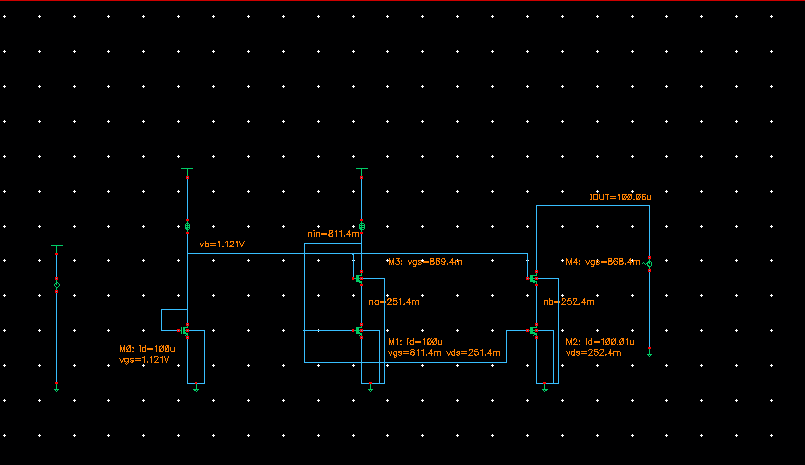
\includegraphics[width=\columnwidth]{fig_sch.png}
\caption{Cadence Virtuoso schematic with the simulated DC operating point
annotated ($V_B=\SI{1.121}{\volt}$, node na = \SI{251}{\milli\volt},
$I_{OUT}=\SI{100.06}{\micro\ampere}$).}
\label{fig:sch}
\end{figure}

\section{Simulation Methodology}
The schematic was simulated with Spectre (NN corner). The DC operating point
was verified device by device; the output voltage was swept
\SIrange{0}{1.8}{\volt} to measure compliance; an AC analysis on the output
source measured the small-signal output impedance; a transient analysis
applied a \SI{100}{\milli\volt}, \SI{1}{\kilo\hertz} sine at the output; and
the supply was swept \SIrange{0}{1.8}{\volt}. In a second deck, simple,
conventional-cascode and high-swing mirrors --- all from identical devices at
\SI{100}{\micro\ampere} --- share one swept output variable so the three
compliance curves superimpose exactly (Fig.~\ref{fig:cmp}).

\section{Results and Discussion}

\subsection{Operating point}
All five devices operate in saturation: M0 at $V_{GS}=\SI{1.121}{\volt}$
($V_{ov}=\SI{0.645}{\volt}\approx2\times$ the mirror overdrive), M1/M2 at
$V_{GS}=\SI{811}{\milli\volt}$ with $V_{DS}\approx\SI{251}{\milli\volt}$, and
the cascodes at $V_{GS}\approx\SI{869}{\milli\volt}$. The output current is
\SI{100.06}{\micro\ampere} at $V_{OUT}=\SI{0.9}{\volt}$ --- a 0.06\%
mirroring error.

\subsection{Topology comparison}
\begin{figure}[!t]
\centering
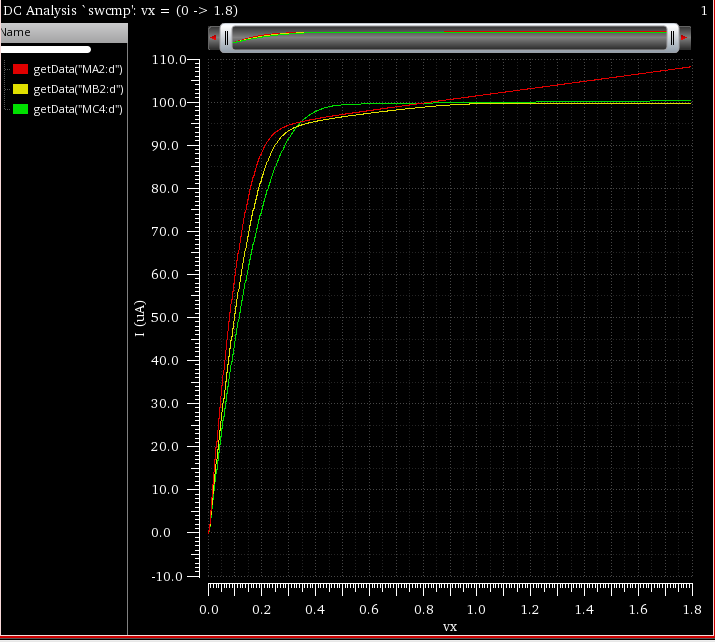
\includegraphics[width=\columnwidth]{fig_cmp.png}
\caption{Output current vs output voltage for the simple mirror (red),
conventional cascode (yellow) and high-swing cascode (green), all at
\SI{100}{\micro\ampere}. The high-swing curve is both flat and early.}
\label{fig:cmp}
\end{figure}

\begin{table}[!t]
\caption{Measured Comparison of the Three Topologies}
\label{tab:cmp}
\centering
\begin{tabular}{lccc}
\toprule
Metric & Simple & Conv. cascode & High-swing \\
\midrule
$V_{OUT}$ for 95\% $I_{OUT}$ & \SI{0.31}{\volt} & \SI{0.35}{\volt} & \SI{0.34}{\volt} \\
$V_{OUT}$ for 99\% $I_{OUT}$ & \SI{0.68}{\volt} & \SI{0.79}{\volt} & \SI{0.44}{\volt} \\
$R_{out}$ (slope 1--1.7 V) & \SI{0.12}{\mega\ohm} & \SI{4.67}{\mega\ohm} & \SI{1.79}{\mega\ohm} \\
$I_{OUT}$ error at \SI{1.8}{\volt} & +8.4\% & +0.001\% & +0.5\% \\
\bottomrule
\end{tabular}
\end{table}

The simple mirror reaches 95\% quickly but never flattens --- its current is
8.4\% high at \SI{1.8}{\volt} and its output resistance is only
\SI{0.12}{\mega\ohm}. The conventional cascode is extremely flat but needs
\SI{0.79}{\volt} before reaching 99\% of the target. The high-swing mirror
achieves 99\% at just \SI{0.44}{\volt} --- saving
$\SI{0.35}{\volt}\approx V_{TH}$ of headroom --- while raising output
resistance $13\times$ over the simple mirror. Its $R_{out}$ is lower than the
conventional cascode's because its bottom devices operate at the saturation
edge ($V_{DS}\approx V_{ov}$), where $g_{ds}$ is larger --- the classic
swing-versus-gain trade, bought deliberately for the headroom.

\subsection{Output compliance and output resistance}
\begin{figure}[!t]
\centering
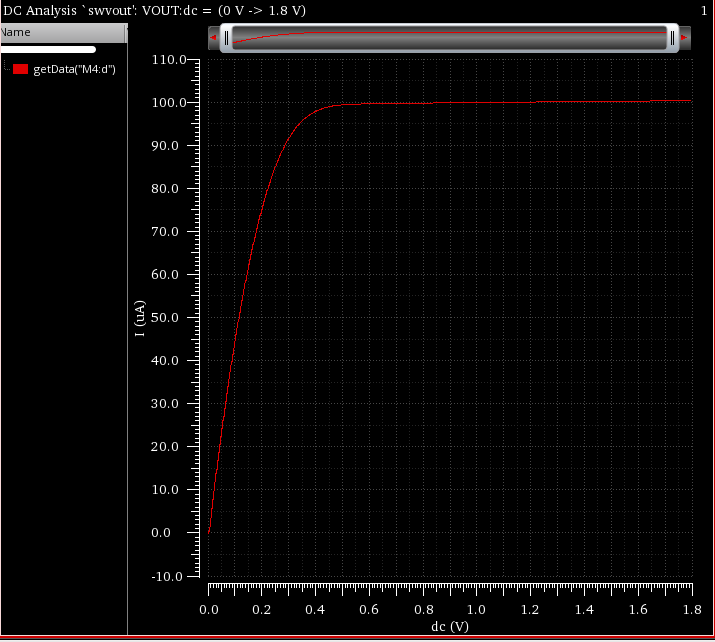
\includegraphics[width=\columnwidth]{fig_vout.png}
\caption{$I_D(\mathrm{M4})$ versus swept output voltage: 92\% at
\SI{0.3}{\volt}, 98\% at \SI{0.4}{\volt}, 99.8\% at \SI{0.6}{\volt}.}
\label{fig:vout}
\end{figure}
\begin{figure}[!t]
\centering
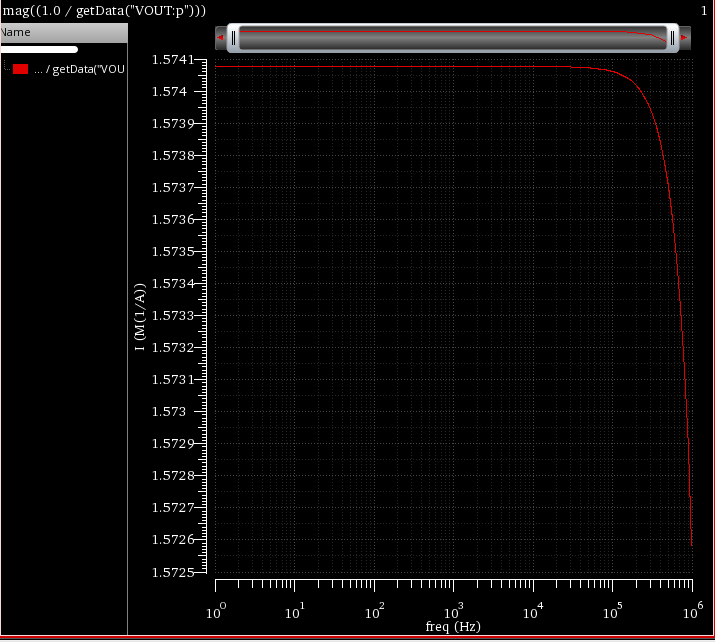
\includegraphics[width=\columnwidth]{fig_rout.png}
\caption{Small-signal output impedance $|V/I|$ from AC analysis:
\SI{1.574}{\mega\ohm}, flat to ${\approx}\SI{100}{\kilo\hertz}$.}
\label{fig:rout}
\end{figure}
The AC measurement (Fig.~\ref{fig:rout}) gives
$R_{out}=\SI{1.574}{\mega\ohm}$ at \SI{1}{\kilo\hertz}, in agreement with the
small-signal estimate $r_{o4}(1+g_{m4}r_{o2})\approx\SI{1.3}{\mega\ohm}$ and
with the DC slope (\SI{1.79}{\mega\ohm}). The roll-off above
\SI{100}{\kilo\hertz} is the output capacitance of M4.

\subsection{Transient behaviour}
\begin{figure}[!t]
\centering
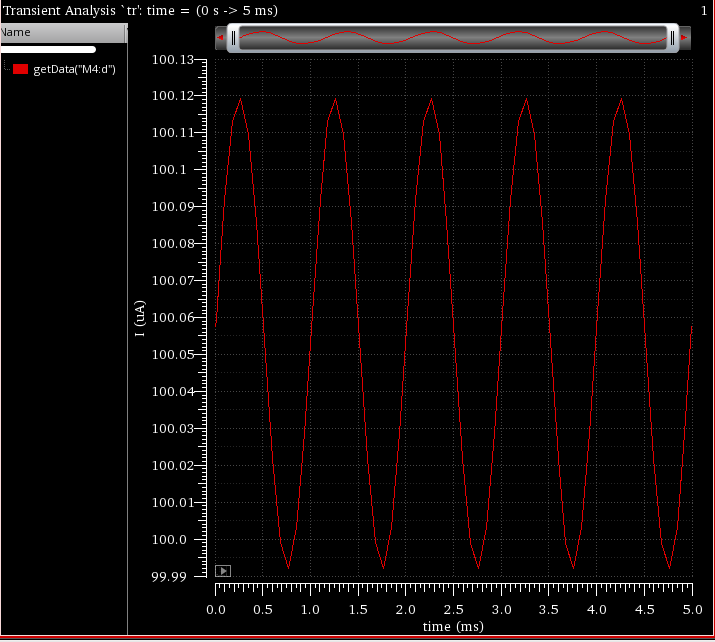
\includegraphics[width=\columnwidth]{fig_tran.png}
\caption{Transient output current with a \SI{100}{\milli\volt},
\SI{1}{\kilo\hertz} sine on the output node: \SI{127}{\nano\ampere}
peak-to-peak ripple about \SI{100.06}{\micro\ampere}.}
\label{fig:tran}
\end{figure}
With a \SI{100}{\milli\volt}-peak disturbance on the output node the mirrored
current ripples only \SI{127}{\nano\ampere} peak-to-peak (0.13\%), equivalent
to $R_{out}=\SI{0.2}{\volt}/\SI{127}{\nano\ampere}=\SI{1.57}{\mega\ohm}$ ---
confirming the AC result in the time domain and demonstrating stable current
operation.

\subsection{Supply sweep}
\begin{figure}[!t]
\centering
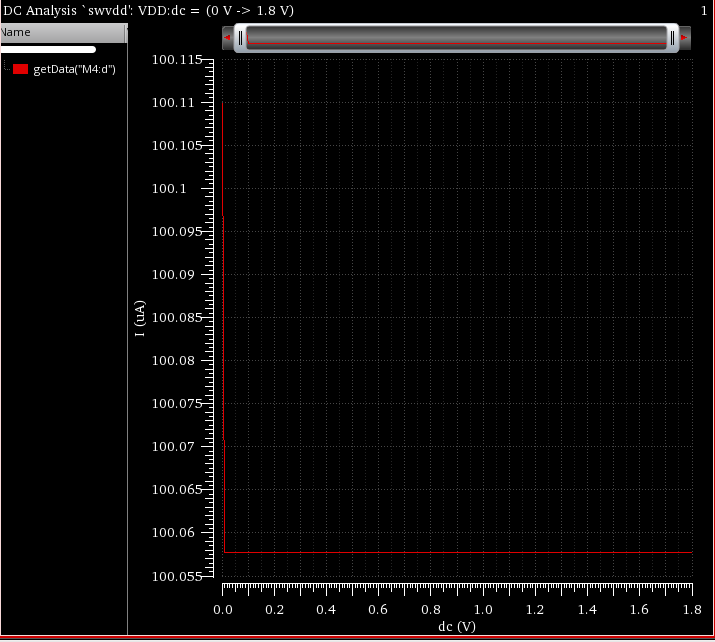
\includegraphics[width=\columnwidth]{fig_vdd.png}
\caption{Output current versus supply voltage at $V_{OUT}=\SI{0.9}{\volt}$:
with the reference branches biased, $I_{OUT}$ varies less than 0.06\% over
the full sweep --- supply-insensitive operation.}
\label{fig:vdd}
\end{figure}

\section{Layout and Physical Verification}
The five-transistor core was laid out in
${\approx}17\times\SI{31}{\micro\metre}$ (Fig.~\ref{fig:layf}): M0, M1, M2 in
the bottom row with integrated body ties (all sources grounded), M3 and M4
stacked above with no local taps (their sources sit at
${\approx}\SI{251}{\milli\volt}$; bulk reaches ground through the substrate).
M3 uses the pcell's switchSD option so its source column lands directly over
M1's drain column, making the na connection a single vertical strap
(Fig.~\ref{fig:laym}). The gate bus of M1/M2 (the IIN net) crosses the na
strap on a short Metal2 bridge with Via1 contacts --- the only use of a
second metal; everything else is Metal1. Diva DRC reports zero errors;
extraction recognizes all five devices; and LVS declares ``The net-lists
match'' with zero unmatched instances, nets, terminals, and zero size errors
(Table~\ref{tab:pv}).

\begin{figure}[!t]
\centering
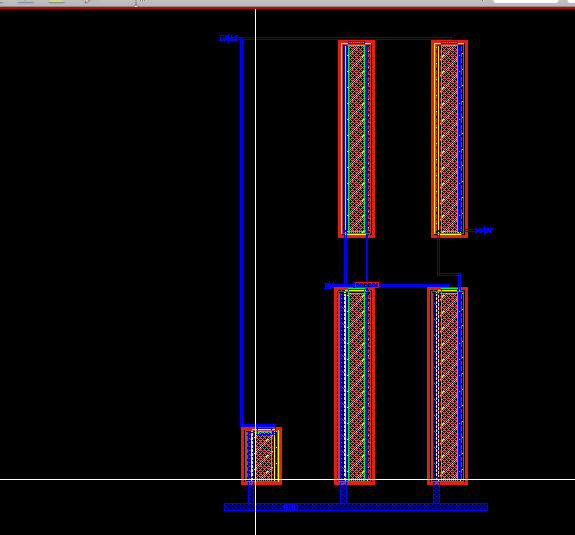
\includegraphics[width=\columnwidth]{fig_layf.png}
\caption{Complete layout: bottom row M0 ($W=\SI{3}{\micro\metre}$), M1, M2;
top row cascodes M3, M4; $V_B$ bus at top, GND rail at bottom.}
\label{fig:layf}
\end{figure}
\begin{figure}[!t]
\centering
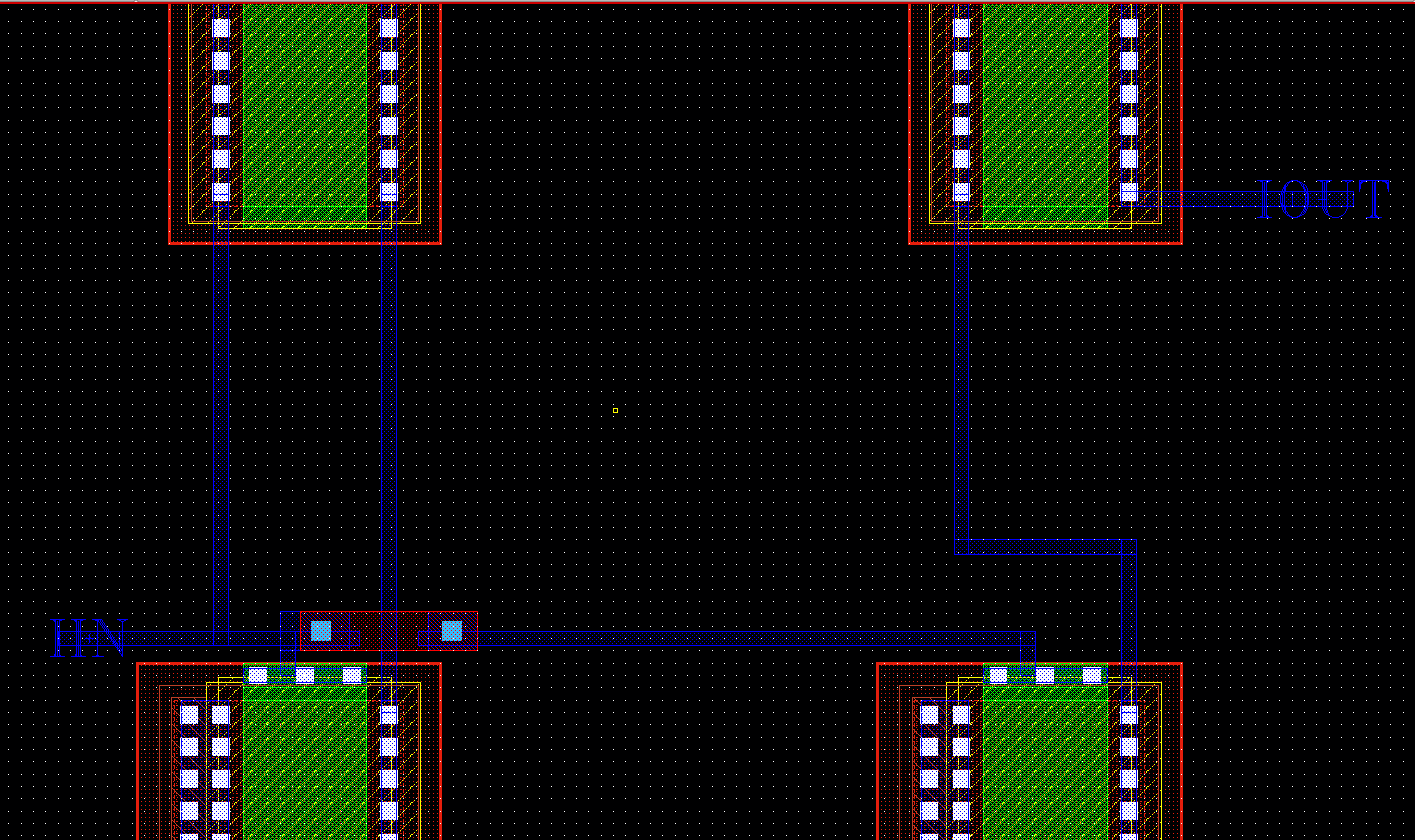
\includegraphics[width=\columnwidth]{fig_laym.png}
\caption{Mid-region detail: the vertical na/nb straps between rows, the IIN
gate bus, and the Metal2 bridge with Via1 pads.}
\label{fig:laym}
\end{figure}

\begin{table}[!t]
\caption{Physical Verification Summary}
\label{tab:pv}
\centering
\begin{tabular}{ll}
\toprule
Check & Result \\
\midrule
Diva DRC & 0 errors \\
Extraction & 5 nmos2v devices, 0 errors \\
LVS verdict & ``The net-lists match'', 0 size errors \\
\bottomrule
\end{tabular}
\end{table}

\section{Advantages, Limitations, and Applications}
The high-swing cascode delivers cascode-class output resistance at nearly the
theoretical minimum compliance voltage, making it the standard mirror for
low-voltage analog design --- op-amp loads, bias distribution and DAC current
sources. Its costs are one extra bias branch (here \SI{100}{\micro\ampere};
in practice the bias device can be scaled to a fraction of the reference),
sensitivity of the $V_{TH}+2V_{ov}$ bias to process and body effect (the
$W/4$ rule is exact only for ideal square-law devices --- margin must be
verified against the technology models, as done here), and a somewhat lower
$R_{out}$ than the conventional cascode because the bottom devices sit at the
saturation edge.

\section{Conclusion}
A high-swing cascode current mirror was designed in Cadence Virtuoso with the
GPDK090 library and verified against BSIM3v3 models at \SI{100}{\micro\ampere}
and \SI{1.8}{\volt}. The quarter-width bias device sets the cascode gates at
$V_{TH}+2V_{ov}=\SI{1.121}{\volt}$, placing the mirror devices at the
saturation edge. Measured against the simple and conventional-cascode mirrors
in one simulation, the design achieves $R_{out}=\SI{1.57}{\mega\ohm}$
($13\times$ the simple mirror) with 99\% compliance at \SI{0.44}{\volt}
(\SI{0.35}{\volt} better than the conventional cascode), and holds its
current within 0.13\% under a \SI{100}{\milli\volt} output disturbance. The
layout passes DRC cleanly and matches the schematic in LVS, completing the
design through physical verification.

\begin{thebibliography}{1}
\bibitem{gray}
P.~R. Gray, P.~J. Hurst, S.~H. Lewis, and R.~G. Meyer, \emph{Analysis and
Design of Analog Integrated Circuits}, 5th~ed. Hoboken, NJ, USA: Wiley, 2009.
\bibitem{razavi}
B.~Razavi, \emph{Design of Analog CMOS Integrated Circuits}, 2nd~ed. New
York, NY, USA: McGraw-Hill, 2017.
\bibitem{sooch}
N.~S. Sooch, ``MOS Cascode Current Mirror,'' U.S. Patent 4,550,284,
Oct.~29, 1985.
\end{thebibliography}

\end{document}
